\documentclass[a4paper,11pt]{article}
\usepackage[a4paper,margin=0.3cm,rmargin=1cm]{geometry}
\usepackage{graphicx}
\usepackage{parskip}
\usepackage{enumitem}
\usepackage{csquotes}
\usepackage{hyperref}
\usepackage{xcolor}
\usepackage{avant} % for font
\usepackage{titlesec}

\renewcommand{\familydefault}{\sfdefault}
\newcommand{\col}[2]{\textcolor[HTML]{#1}{#2}}

\titlespacing*{\section}{0pt}{12pt}{6pt}

% rm left indent
\setlength{\parindent}{0pt}

% compact enumerations
\setlist{noitemsep,topsep=0pt,leftmargin=*}
% \setitemize{noitemsep,topsep=0pt,parsep=0pt,partopsep=0pt}

% include path for images
\graphicspath{ {./images/} }

\begin{document}

% banner on left side
\noindent
\begin{minipage}[t]{0.3106\textwidth}
    \clearpage  % fix for page break before content
    \vspace{-0.45cm}
    
\includegraphics[width=\textwidth]{triangles.pdf}
    \begin{center}
    \tiny \col{316dbc}{made with \href{https://github.com/louisradtke/cv-banner}{github.com/louisradtke/cv-banner}}
    \end{center}

    % profile picture
    \vspace{-26.92cm}
    \begin{center}
        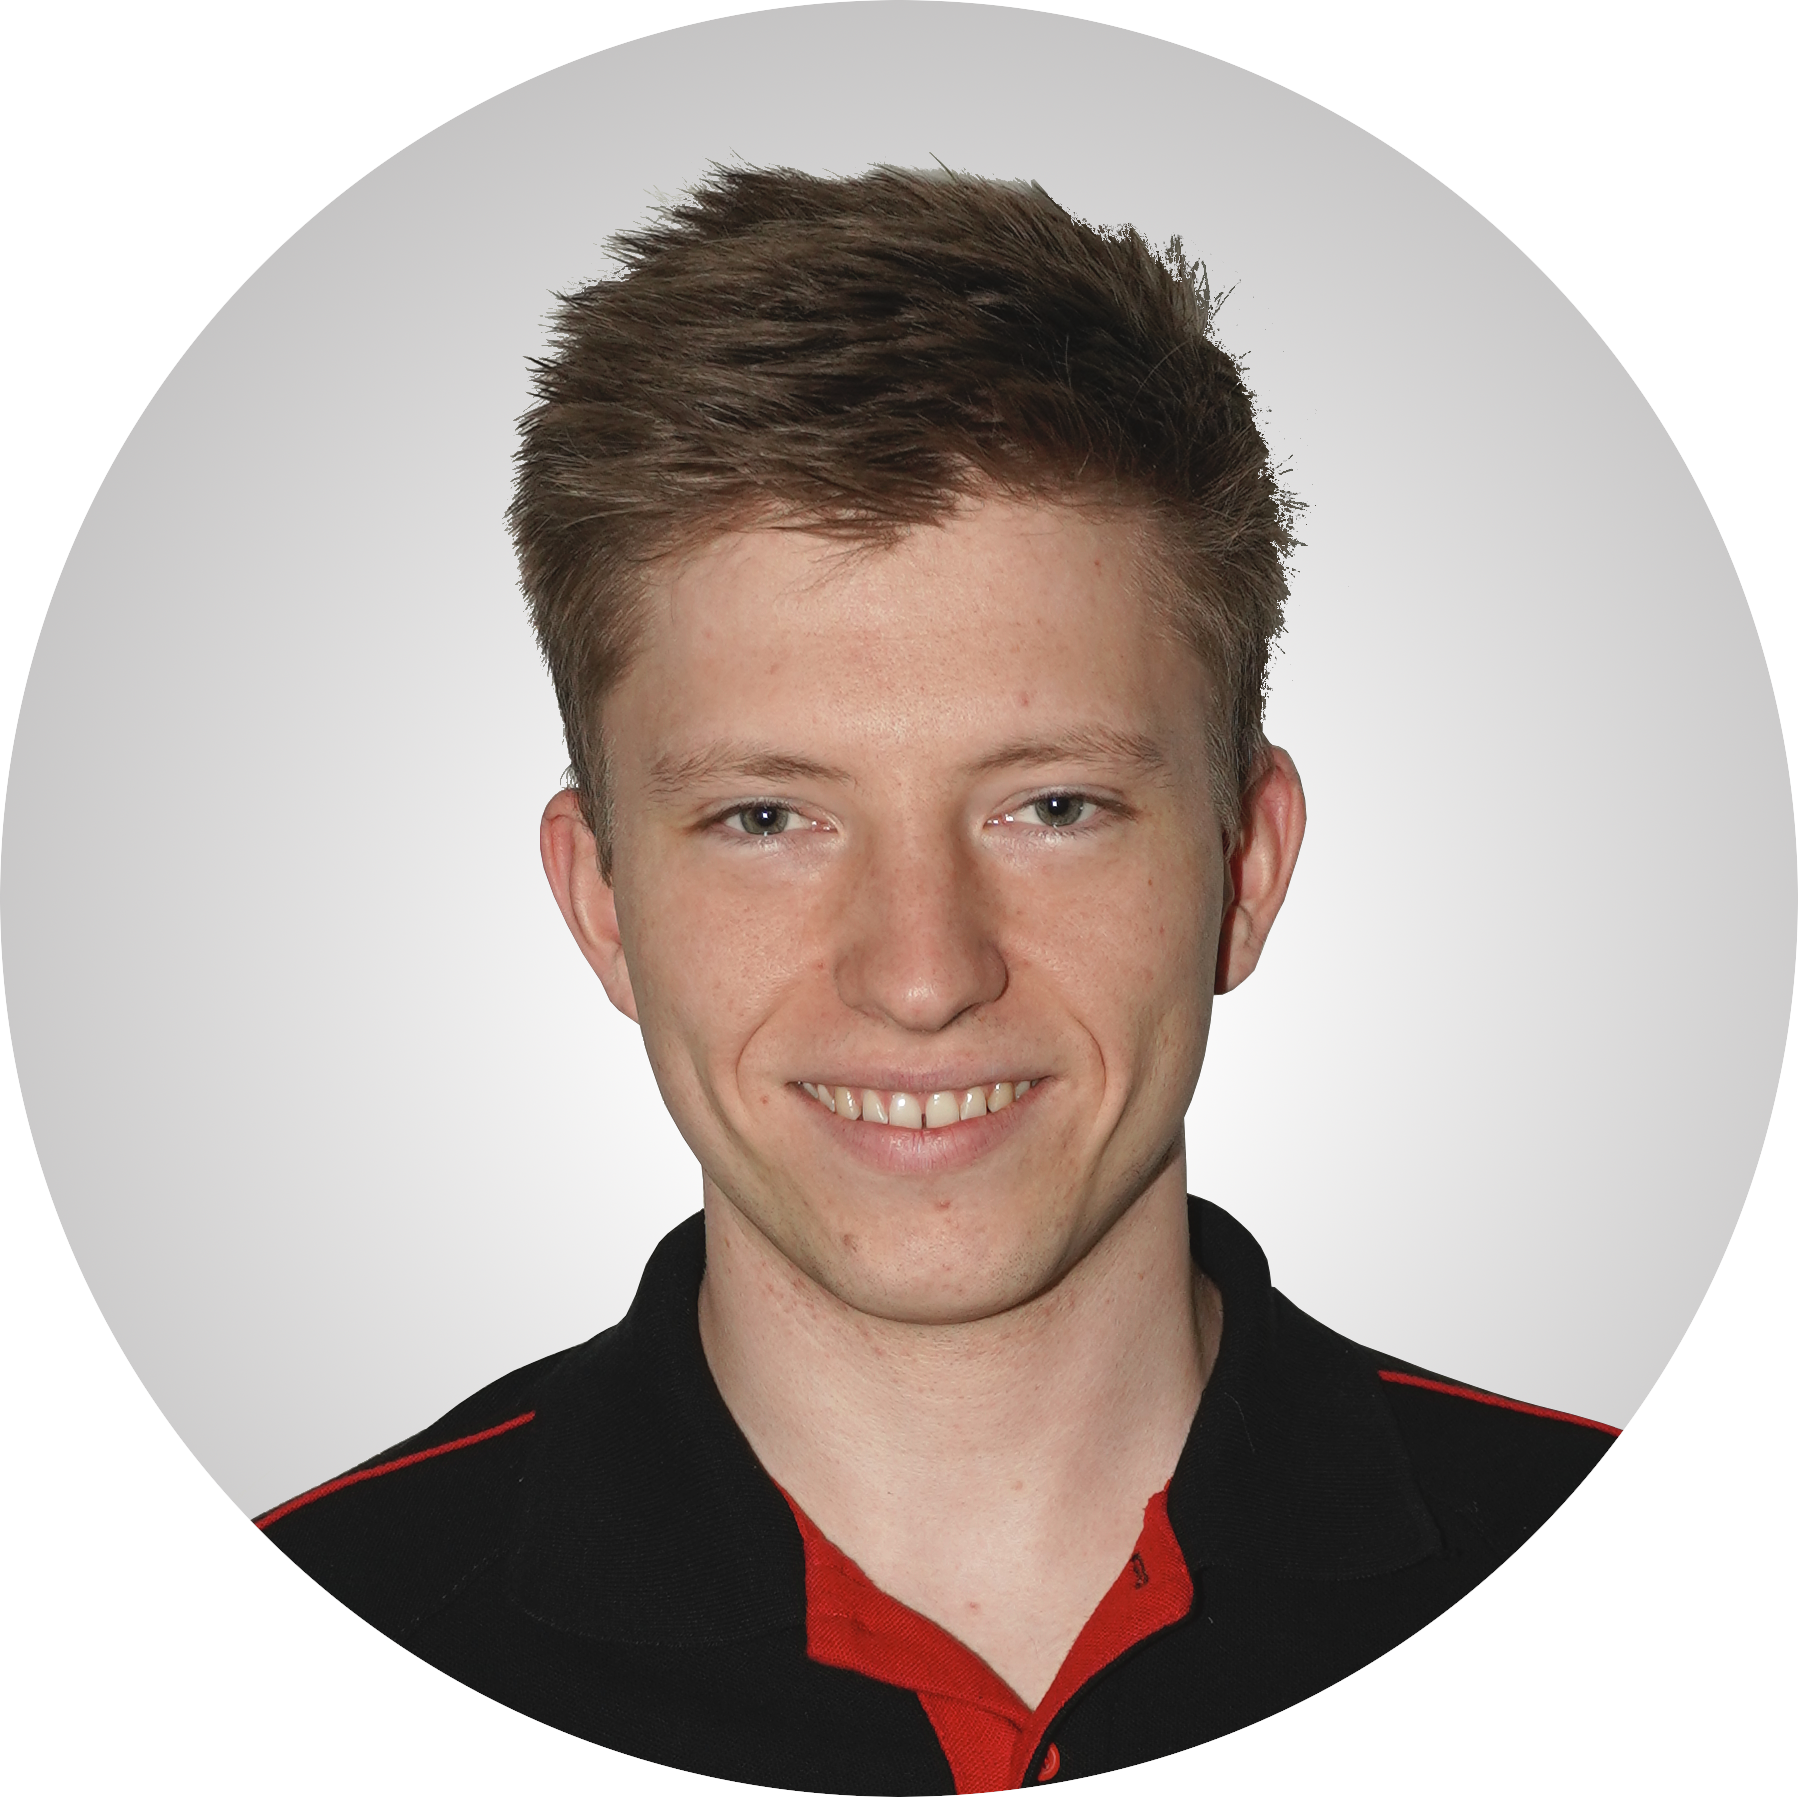
\includegraphics[width=4.5cm,clip]{profile.png}
    \end{center}

    \vspace{2.15cm}
    \begin{center}
    \begin{minipage}{0.72\textwidth}
        % \centering
        % \textsc{\textbf{Louis Radtke}}\\
        % \huge\col{c6997c}{\textbf{Louis Radtke}}\\
        \huge\textbf{Louis Radtke}\\
        \scriptsize born January 1999, Hagen, DE\\
        louisradtke.dev@gmail.com\\
        \url{https://louisradtke.dev}
        % \normalsize software engineer\\
        % robotics engineer
    \end{minipage}
    \end{center}

    % text block 1:
    % Louis Radtke, B.Sc.
    % sth. w/ software engineer, robotics engineer, workflow optimizer, team player

    % footer for flow: made with github.com/louisradtke-cv-flow
\end{minipage}
\hfill
\begin{minipage}[t]{0.65\textwidth}
    \vspace{0cm}
    \begin{center}
        \title*{\Huge \textsc{\textbf{Curriculum Vitae}}}
        % \title*{\Huge \col{c67e43}{\textsc{\textbf{Curriculum Vitae}}}}
    \end{center}

    Lorem ipsum dolor sit amet, consetetur sadipscing elitr, sed diam nonumy eirmod tempor.
    % to do: summary about professional profile. carer goals? highlight of key achievements.

    \vspace{0.5cm}
    \hrule

    \section*{\col{ac7448}{Experience}}
    \col{b27c52}{\textbf{Research Assistant \hfill 2024 -- Today}}\\
    AQUA Research Group, TU Dortmund, DE
    \begin{itemize}
        \small
        \item Preparation of the research data infrastructure.
        \item Support in procurement of an FSD testing vehicle.
    \end{itemize}

    \vspace{0.2cm}

    \col{b3805b}{\textbf{Software Engineer \hfill 2018 -- Today}} \\
    SimPlan Integrations GmbH, Witten, DE
    \begin{itemize}
        \small
        \item Key responsibility or achievement 1.
        \item Key responsibility or achievement 2.
    \end{itemize}

    \vspace{0.2cm}

    \col{b38668}{\textbf{Team Captain / CEO \hfill 2023}} \\
    GET racing, Formula Student Team of TU Dortmund, DE
    \begin{itemize}
        \small
        \item Coordination of the production phase of the FS223 vehicle.
        \item Commissioning and integration of autonomous driving software.
        \item Logistical planning of the competitions.
    \end{itemize}

    \vspace{0.2cm}

    \textbf{\col{a68573}{Autonomous System Lead \hfill 2019 -- 2023}} \\
    GET racing, Formula Student Team of TU Dortmund, DE
    \begin{itemize}
        \small
        \item Initial assembly of the autonomous system department.
        \item Acquisition of partners in industry and at university.
        \item Conception and implementation of the autonomous system software.
        \item Commissioning and development of automated simulation infrastructure.
        \item Introduction of new PM tool (JetBrains YouTrack) to entire team.
        \item Maintaining online services and network infrastructure.
    \end{itemize}

    \section*{\col{908587}{Education}}
    \col{91878a}{\textbf{M.Sc. in Computer Science \hfill 2022 -- Today}} \\
    TU Dortmund, DE
    \begin{itemize}
        \small
        \item Seminar: AI in Software Engineering -- built RAG pipeline using LLMs
        \item Project group: \enquote{Continuous and Compositional Validation}
        \item Research project: building a research data management system
        \item Courses on software engineering, computer graphics, pattern recognition, real time operating systems and deep \& reinforcement learning (AI)
    \end{itemize}

    \vspace{0.2cm}

    \col{81879c}{\textbf{B.Sc. in Computer Science \hfill 2017 -- 2022}} \\
    TU Dortmund, DE
    \begin{itemize}
        \small
        \item Minor subject: Robotics (controls theory and electronics)
        \item Thesis: A method for localizing mobile robots using multiple sensors
    \end{itemize}

    \vspace{0.2cm}

    \col{81879c}{\textbf{Abitur \hfill 2009 -- 2017}} \\
    Gymnasium Hohenlimburg, Hagen, DE

    \begin{minipage}[t]{0.65\textwidth}
        \col{7690bb}{\section*{Skills}}
        \begin{itemize}
            \small
            \item Programming \& Ecosystems:\\
            .NET (++++), Python (++++), C++ (+++),\\
            JS/TS (++), Java/Kotlin (++)
            \item Systems \& Administration:\\
            Linux
            \item Project Management Tools:\\
            GitLab (++++), YouTrack ()
            \item Skill 3
            \item Skill 4
            \item Skill 5
            \item Skill 6
            \item Skill 7
            \item Skill 8
        \end{itemize}
    \end{minipage}
    \hfill
    \begin{minipage}[t]{0.3\textwidth}
        \col{ffffff}{.} % dirty fix for v misalignment of headings
        \section*{\col{7690bb}{Languages}}
        \begin{itemize}
            \small
            \item German -- Native
            \item English -- Fluent
            \item French -- Basic
        \end{itemize}
    \end{minipage}

\end{minipage}

\end{document}
